\subsection{Solución}

Para poder levantar la base de datos por medio de archivos de texto, lo principal es normalizar la base del archivo "Universidad.xls". Posterior a esto, debemos migrar los datos que contiene originalmente a la nueva estructura normalizada que se muestra a continuación:

\begin{figure}[H]
    \centering
    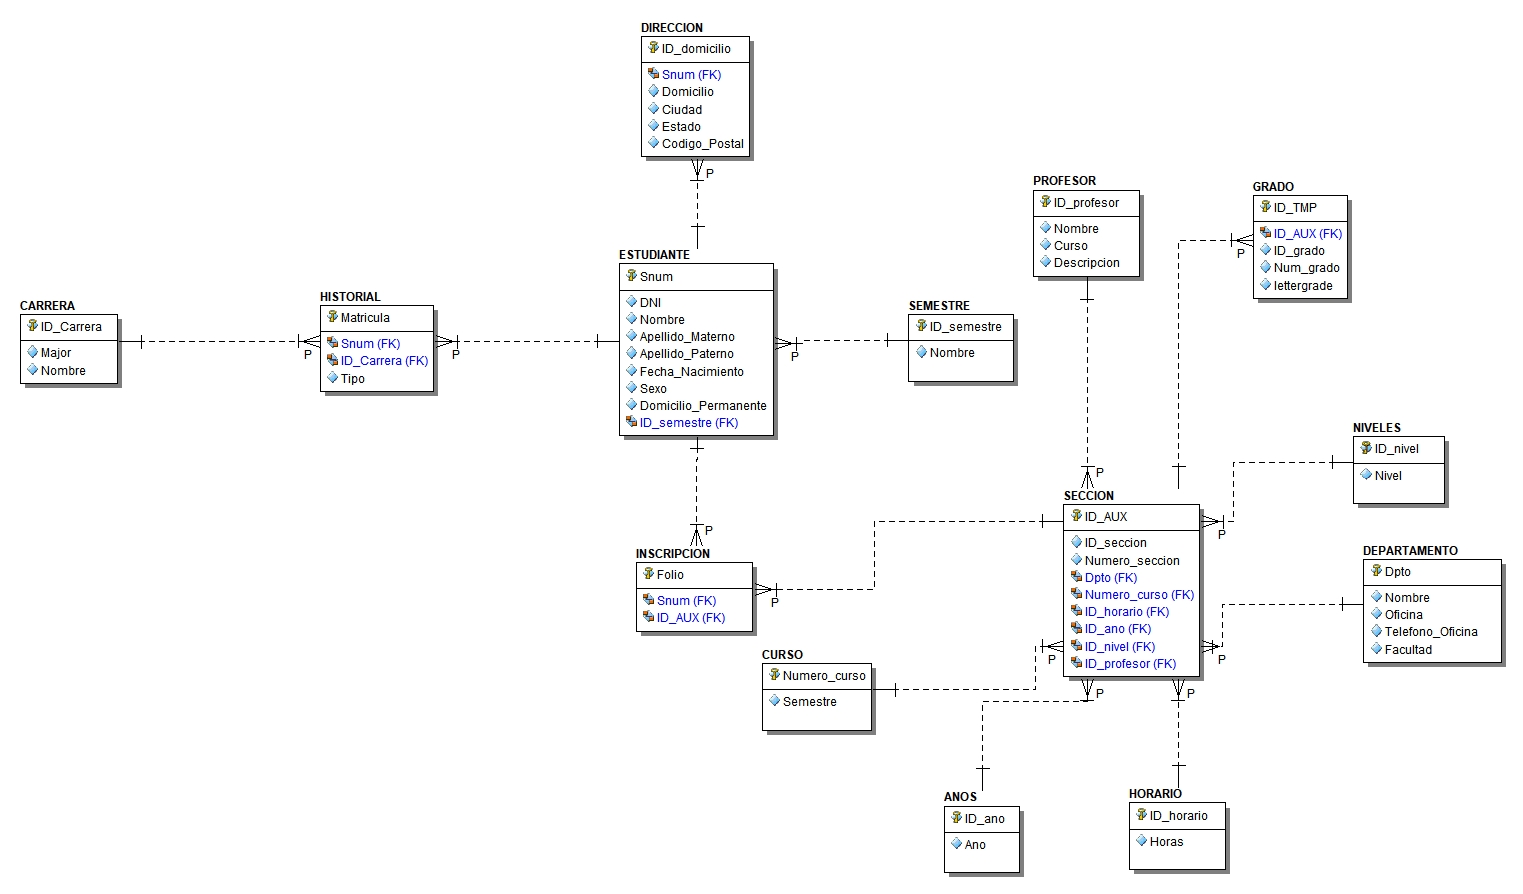
\includegraphics[width=1.0\textwidth]{Diagrama Entidad-Relacion.jpeg} 
    \caption{Diagrama Entidad-Relación}
\end{figure}

Con esto podemos identificar varios elementos importantes: son 14 tablas, las cuales debemos crear como archivos y llenarlas con sus respectivos datos.

\subsubsection{Tabla Estudiantes}
Esta tabla almacena los 20 registros de los estudiantes, su semestre y el domicilio permanente. Esto evita agregar registros vacíos dentro de la tabla dirección, además de ser atributos intrínsecos del estudiante.

\begin{figure}[H]
    \centering
    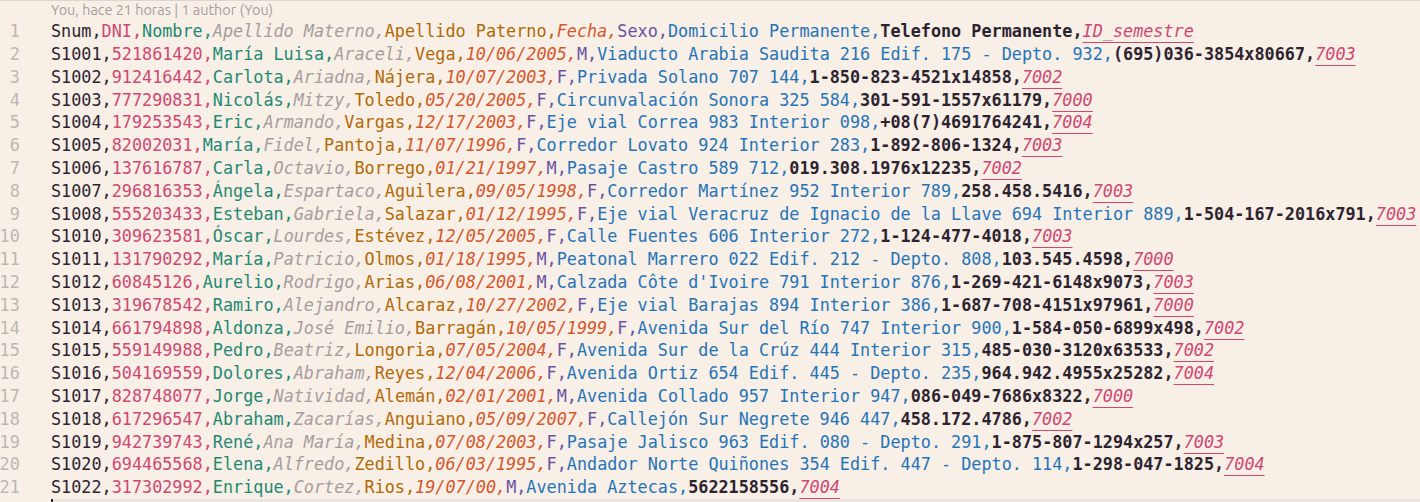
\includegraphics[width=1.0\textwidth]{Estudiantes.png} 
    \caption*{Tabla 1. Estudiante}
\end{figure}

\subsubsection{Tabla Dirección}
Esta tabla almacena la dirección actual del estudiante, la cual es más propensa a ser cambiada y por eso no se agrega directamente a la tabla de estudiantes (a diferencia de su domicilio permanente).

\begin{figure}[H]
    \centering
    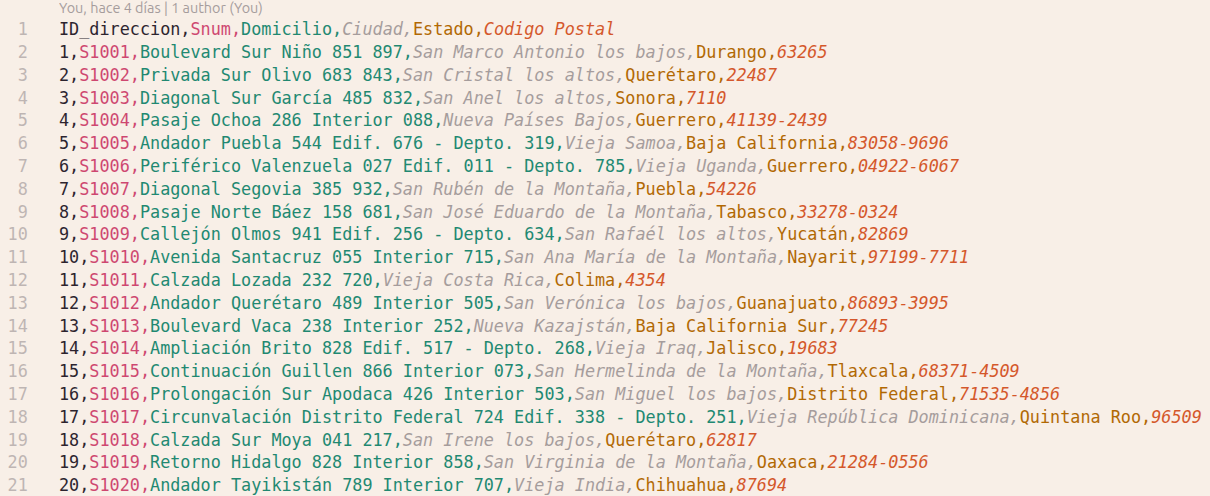
\includegraphics[width=1.0\textwidth]{Direccion.png} 
    \caption*{Tabla 2. Dirección}
\end{figure}

\subsubsection{Tabla Carrera}
La tabla carrera almacena los nombres de cada carrera. Debido a que un estudiante puede cursar una o más carreras, la relación es de muchos a muchos. Esto obliga a generar una tabla intermedia entre el estudiante y las carreras, que se llamará historial.

\begin{figure}[H]
    \centering
    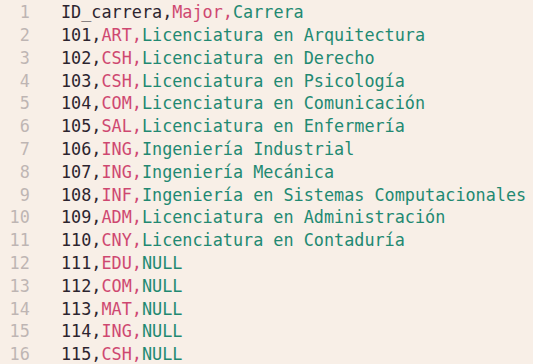
\includegraphics[width=0.40\textwidth]{Carrera.png} 
    \caption*{Tabla 3. Carrera}
\end{figure}

\subsubsection{Tabla Historial}
Esta es la tabla intermedia que se genera entre el estudiante y el catálogo de carreras. Si un registro tiene más de una llave, significa que el alumno cursa más de una carrera.

\begin{figure}[H]
    \centering
    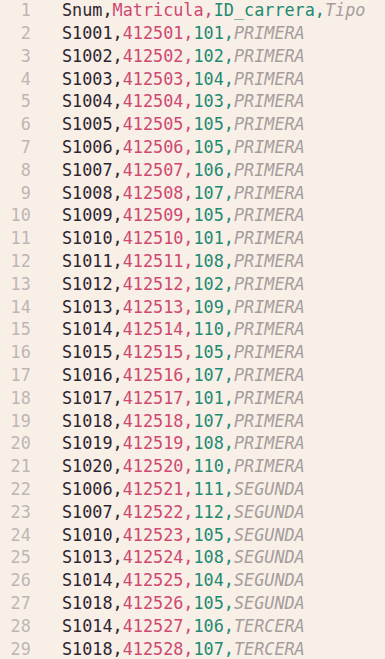
\includegraphics[width=0.32\textwidth]{Historial.png} 
    \caption*{Tabla 4. Historial}
\end{figure}

\subsubsection{Tabla Inscripción}
Esta tabla es el producto de la relación entre el estudiante y la sección en la que está inscrito. Al ser una relación de muchos a muchos, la llamamos inscripción, pues un estudiante puede inscribir una o varias secciones.

\begin{figure}[H]
    \centering
    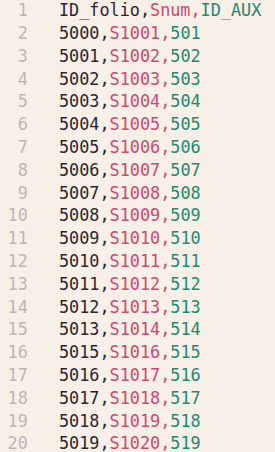
\includegraphics[width=0.28\textwidth]{Inscripcion.png} 
    \caption*{Tabla 5. Inscripción}
\end{figure}

\subsubsection{Tabla Sección}
Esta tabla es la que almacena el registro de la sección inscrita, junto con el profesor y el departamento que la imparte, además de su calificación definida.

\begin{figure}[H]
    \centering
    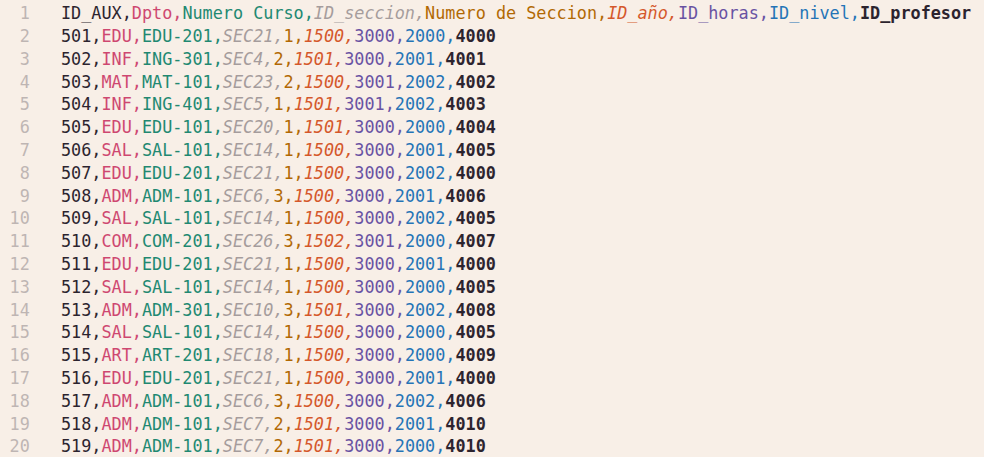
\includegraphics[width=0.75\textwidth]{Seccion.png} 
    \caption*{Tabla 6. Sección}
\end{figure}

\subsubsection{Tabla Profesor}
La tabla profesor almacena el nombre, el curso y una breve descripción de la asignatura que imparte el docente en una o varias secciones.

\begin{figure}[H]
    \centering
    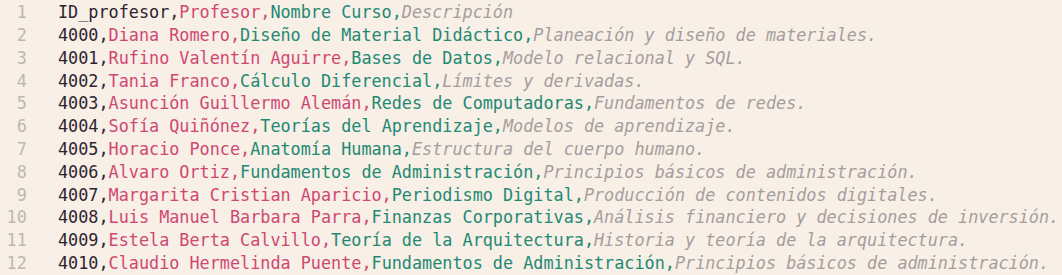
\includegraphics[width=1.0\textwidth]{Profesor.png} 
    \caption*{Tabla 7. Profesor}
\end{figure}

\subsubsection{Tabla Departamento}
El departamento contiene los nombres de cada uno, su abreviatura, un teléfono de oficina y la facultad a la que pertenece la sección.

\begin{figure}[H]
    \centering
    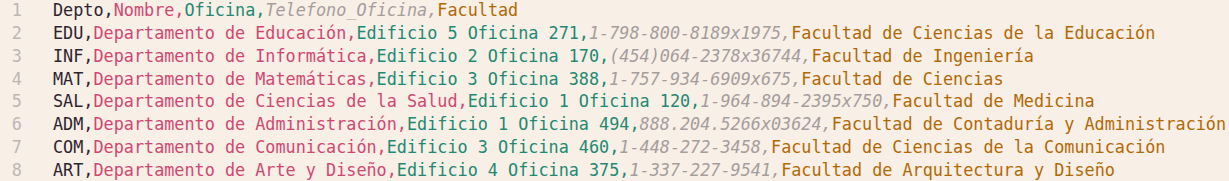
\includegraphics[width=1.0\textwidth]{Departamento.png} 
    \caption*{Tabla 8. Departamento}
\end{figure}

\subsubsection{Tabla Niveles}
Esta tabla solo almacena el nivel en el que se impartió la sección.

\begin{figure}[H]
    \centering
    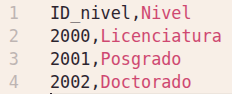
\includegraphics[width=0.35\textwidth]{Niveles.png} 
    \caption*{Tabla 9. Niveles}
\end{figure}

\newpage
\subsubsection{Tabla Horario}
La tabla guarda el número de horas en las que se imparte una sección.

\begin{figure}[H]
    \centering
    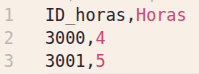
\includegraphics[width=0.25\textwidth]{Horario.png} 
    \caption*{Tabla 10. Horario}
\end{figure}

\subsubsection{Tabla Grado}
La tabla grado almacena la calificación obtenida en una sección.

\begin{figure}[H]
    \centering
    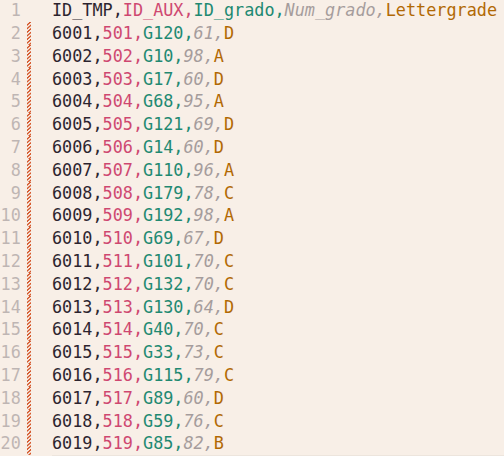
\includegraphics[width=0.40\textwidth]{Grado.png} 
    \caption*{Tabla 11. Grado}
\end{figure}

\subsubsection{Tabla Curso}
La tabla curso almacena la estación del año en la que se imparte la sección y el salón asignado.

\begin{figure}[H]
    \centering
    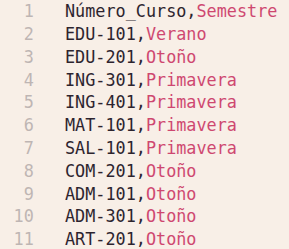
\includegraphics[width=0.30\textwidth]{Curso.png} 
    \caption*{Tabla 12. Curso}
\end{figure}

\subsubsection{Tabla Años}
La tabla años solo almacena el año en el que se impartió la sección.

\begin{figure}[H]
    \centering
    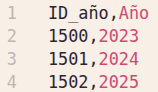
\includegraphics[width=0.25\textwidth]{Años.png} 
    \caption*{Tabla 13. Años}
\end{figure}

\subsubsection{Tabla Semestre}
Esta tabla solo almacena el semestre en el que se encuentra el estudiante.

\begin{figure}[H]
    \centering
    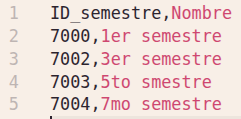
\includegraphics[width=0.35\textwidth]{Semestre.png} 
    \caption*{Tabla 14. Semestre}
\end{figure}